\documentclass[12pt,a4paper]{article}
\usepackage[utf8]{inputenc}
\usepackage[T1]{fontenc}
\usepackage[spanish,es-tabla]{babel}
\usepackage{graphicx}
\usepackage{float}
\usepackage{geometry}
\usepackage{hyperref}
\usepackage{fancyhdr}
\usepackage{titlesec}
\usepackage{booktabs}
\usepackage{array}
\usepackage{longtable}
\usepackage{xcolor}
\usepackage{mathptmx}
\usepackage{amsmath}
\usepackage{setspace}
\usepackage{xurl}

\geometry{top=2.5cm, bottom=2.5cm, left=3cm, right=3cm}
\hypersetup{colorlinks=true, linkcolor=black, urlcolor=blue, citecolor=black}
\graphicspath{{data/}{outputs/}}

\pagestyle{fancy}
\fancyhf{}
\fancyhead[L]{\small Corte 2: algoritmos de búsqueda}
\fancyhead[R]{\thepage}
\renewcommand{\headrulewidth}{0.4pt}
\setlength{\headheight}{14.5pt}
\setlength{\emergencystretch}{3em}

\titleformat{\section}{\normalfont\Large\bfseries}{\thesection}{1em}{}
\titleformat{\subsection}{\normalfont\large\bfseries}{\thesubsection}{1em}{}

\begin{document}

\begin{titlepage}
\thispagestyle{empty}
\centering

\vspace*{0.5cm}

\includegraphics[width=0.30\textwidth]{sergio_logo.png}\\[0.4cm]

{\fontsize{13}{15}\selectfont\textbf{UNIVERSIDAD SERGIO ARBOLEDA}}\\[2.0cm]

{\fontsize{14}{17}\selectfont\textbf{ALGORITMOS DE BÚSQUEDA SOBRE UNA RED DE\\
CARGA INTERURBANA: BFS, DFS, COSTO UNIFORME,\\
VORAZ Y A*}}\\[0.6cm]
{\fontsize{12}{14}\selectfont Proyecto Integrador, Corte 2}\\[2.2cm]

{\fontsize{12}{14}\selectfont\textbf{Inteligencia Artificial (SIST5036)}}\\[1.5cm]

{\fontsize{12}{14}\selectfont
Juan David Andradé Gómez\\[0.2cm]
Mario Jiménez López\\[0.2cm]
Camilo Andrés Díaz García}\\[1.2cm]

{\fontsize{12}{14}\selectfont Profesor: Joaquín F. Sánchez}

\vfill

\begin{center}
    \textit{Universidad Sergio Arboleda}\\
    \textit{Facultad de Sistemas e Ingeniería}\\
    \textit{Bogotá D.C., 2026}
\end{center}

\end{titlepage}

\newpage
\tableofcontents
\newpage

\section{Formulación de continuidad}

La formulación del problema, los datos y su construcción están en el informe
del Corte 1~\cite{formulacion}. La red corregida a la que se refiere este
informe tiene 32 nodos, porque se excluyó Mosquera, y 9 registros con la
distancia corregida por doble calzada digitalizada; ambos cambios se
documentan en ese informe. Como problema
de búsqueda, el estado es la ciudad actual; las acciones son los tramos que
salen de ella; el costo de una acción es el atributo de la arista según el
criterio (\texttt{distancia}, \texttt{compuesto\_sin\_riesgo},
\texttt{compuesto} o \texttt{riesgo}); y la meta es la ciudad de destino. En el
caso central, Duitama a Puente Nacional, las dos rutas miden 309.10 km por
Bogotá y 654.25 km por Santander. El sector de Chocontá a Tunja está truncado
en la fuente (17.69 km frente a 56.96 km de línea recta), por lo que la ruta
por Bogotá tiene una cota inferior de $309.10 - 17.69 + 56.96 = 348.37$ km
(cota inferior: la geodésica no excede la distancia por carretera; no es un
valor estimado), y de esa arista depende el valor de $\alpha$ de la
Sección~\ref{sec:heuristica}.

\section{Implementación de los cinco algoritmos}

Los algoritmos están en \texttt{src/busquedas.py}, programados desde cero: el
grafo solo aporta vecinos y costos, y no se usa ninguna búsqueda de
\texttt{networkx} (para poder contar nodos expandidos).

\begin{table}[H]
\centering
\caption{Los cinco algoritmos}
\label{tab:algoritmos}
\small
\begin{tabular}{>{\raggedright\arraybackslash}p{2.2cm}>{\raggedright\arraybackslash}p{4.2cm}>{\raggedright\arraybackslash}p{6.3cm}}
\toprule
\textbf{Algoritmo} & \textbf{Frontera} & \textbf{Resultado garantizado} \\
\midrule
BFS & Cola FIFO & Mínimo número de saltos, no mínimo costo \\
DFS & Pila LIFO & Primera ruta que encuentra; sin garantía \\
UCS & Cola de prioridad por $g(n)$ & Óptimo para costos no negativos \\
Voraz & Cola de prioridad por $h(n)$ & Sin garantía de optimalidad \\
A* & Cola de prioridad por $g(n)+h(n)$ & Óptimo si $h$ es admisible \\
\bottomrule
\end{tabular}
\end{table}

Convenciones comunes, para que los contadores sean comparables: la prueba de
meta se hace al extraer el nodo de la frontera; \emph{nodos expandidos} son los
extraídos cuyos sucesores se generan (la meta no se cuenta); \emph{nodos
generados} son los insertados en la frontera; y los vecinos se recorren en
orden alfabético, de modo que BFS y DFS son deterministas. UCS y A* admiten
reexpansión de un nodo si su costo mejora; con una heurística consistente no
ocurre. Todos devuelven la ruta, el costo, los nodos expandidos y generados y
el tamaño máximo de la frontera.

\textbf{Pruebas de corrección} (\texttt{src/pruebas\_busquedas.py}): un grafo
de juguete con resultado conocido; 600 pares en 25 grafos geométricos
aleatorios con semilla fija; y los 992 pares de nodos de la red con los cinco
criterios. En todos, UCS y A* igualan el costo de
\texttt{nx.shortest\_path\_length}, BFS iguala su número de saltos, y DFS y la
búsqueda voraz devuelven rutas válidas. Todas las pruebas pasan.

\section{Heurística: admisibilidad y consistencia}
\label{sec:heuristica}

Para los criterios basados en distancia se usa
\begin{equation}
h(n) = \alpha\, d_{\mathrm{geo}}(n, \text{meta}), \qquad
h(n) = \frac{w_1}{w_1 + w_2}\,\alpha\,\frac{d_{\mathrm{geo}}(n, \text{meta})}
{d_{\max}}
\end{equation}
para \texttt{distancia} y \texttt{compuesto\_sin\_riesgo}, respectivamente, con
$d_{\mathrm{geo}}$ la distancia de Haversine entre las coordenadas oficiales
(DANE, DIVIPOLA) y $\alpha$ el mínimo de la razón carretera/geodésica entre las
aristas, redondeado hacia abajo a 6 decimales. Con ese $\alpha$,
$\alpha\, d_{\mathrm{geo}}(u,v) \le c(u,v)$ en toda arista, lo que garantiza
admisibilidad y consistencia por la desigualdad triangular. Los términos de
peaje y de riesgo (no negativos) no se incluyen en $h$ y no la rompen.

\textbf{Valor de $\alpha$.} $\alpha = 0.310570$ (razón mínima exacta
0.3105704113). La determina la arista de Chocontá a Tunja, cuyo sector está
truncado en la fuente. Las demás aristas con razón menor que 1 se muestran en
la Tabla~\ref{tab:razones}.

\begin{table}[H]
\centering
\caption{Aristas con razón carretera/geodésica menor que 1}
\label{tab:razones}
\small
\renewcommand{\arraystretch}{1.2}
\begin{tabular}{|l|r|r|r|}
\hline
\rowcolor{gray!20} \textbf{Arista} & \textbf{Carretera (km)} & \textbf{Geodésica (km)} & \textbf{Razón} \\
\hline
\textbf{Chocontá -- Tunja} & 17.69 & 56.96 & 0.310570 \\
\hline
\textbf{Bogotá -- Madrid} & 9.12 & 19.91 & 0.458156 \\
\hline
\textbf{Bogotá -- Tocancipá} & 22.12 & 41.19 & 0.537062 \\
\hline
\textbf{Cajicá -- Zipaquirá} & 9.10 & 12.15 & 0.749212 \\
\hline
\textbf{Granada -- Ye de Granada} & 2.43 & 3.04 & 0.798421 \\
\hline
\textbf{El Espinal -- Girardot} & 19.36 & 20.42 & 0.947938 \\
\hline
\textbf{Bogotá -- Guasca} & 34.88 & 35.12 & 0.993148 \\
\hline
\textbf{Duitama -- Tunja} & 47.73 & 47.78 & 0.998874 \\
\hline
\end{tabular}

\end{table}

\textbf{Verificación numérica} (Tabla~\ref{tab:heuristica}). La admisibilidad
compara $h(n)$ con el costo óptimo real $h^*(n)$ de Dijkstra para los 992
pares $(n, \text{meta})$; la consistencia comprueba $h(u) \le c(u,v) + h(v)$
en cada arista, en ambos sentidos y para las 32 metas. Con $\alpha = 0.310570$
no hay violaciones y el margen mínimo es de 0.000023 km, en Chocontá a Tunja.
Con la geodésica pura ($\alpha = 1$) hay 66 violaciones de admisibilidad y 141
de consistencia: el peor margen es $-56.51$ km.

\begin{table}[H]
\centering
\caption{Verificación de admisibilidad y consistencia (margen mínimo en las
unidades del criterio)}
\label{tab:heuristica}
\small
\setlength{\tabcolsep}{4pt}
\renewcommand{\arraystretch}{1.2}
\begin{tabular}{|l|r|r|r|r|r|}
\hline
\rowcolor{gray!20} \textbf{Heurística} & \textbf{$\alpha$} & \textbf{Viol. adm.} & \textbf{Margen adm.} & \textbf{Viol. cons.} & \textbf{Margen cons.} \\
\hline
\textbf{distancia} & 0.310570 & 0 & 0.000023 & 0 & 0.000023 \\
\hline
\textbf{compuesto sin riesgo} & 0.310570 & 0 & 0.005265 & 0 & 0.005265 \\
\hline
\textbf{compuesto (limitado)} & 0.310570 & 0 & 0.012594 & 0 & 0.012594 \\
\hline
\textbf{costo operativo} & 0.310570 & 0 & 1717.883246 & 0 & 1717.883246 \\
\hline
\textbf{total sin riesgo} & 0.310570 & 0 & 0.007020 & 0 & 0.007020 \\
\hline
\textbf{total (limitado)} & 0.310570 & 0 & 0.018892 & 0 & 0.018892 \\
\hline
\textbf{mortalidad (limitado)} & 0.310570 & 0 & 0.003510 & 0 & 0.003510 \\
\hline
\textbf{distancia, geodésica pura} & 1 & 66 & -56.51 & 141 & -39.27 \\
\hline
\end{tabular}

\end{table}

\textbf{Aristas con carretera menor que la geodésica.} Se reportan todas
(Tabla~\ref{tab:razones}); no se ajustó ninguna distancia para que la
heurística cumpla. Varias se explican por la entrada urbana a Bogotá, que la
geometría de INVÍAS no cubre. Como $\alpha$ es la razón mínima, la
heurística es poco informativa en los corredores donde la carretera es mucho
más larga que la línea recta.

\textbf{Criterios con heurística limitada.} En \texttt{compuesto} (riesgo
faltante igual a 0) se usa solo el término de distancia, $w_1 \alpha
d_{\mathrm{geo}}/d_{\max}$, y los resultados se reportan aparte, rotulados
como limitados. En \texttt{riesgo} y \texttt{peaje} no hay información
geométrica: la heurística admisible es $h = 0$, y A* se reduce a costo
uniforme.

\section{Escenarios}

\begin{table}[H]
\centering
\caption{Escenarios origen-destino}
\label{tab:escenarios}
\small
\setlength{\tabcolsep}{4pt}
\begin{tabular}{lcr>{\raggedright\arraybackslash}p{5.4cm}}
\toprule
\textbf{Escenario} & \textbf{Rutas} & \textbf{Saltos} & \textbf{Motivo} \\
\midrule
Duitama -- Puente Nacional & 2 & 8 & caso central: dos rutas reales \\
Tunja -- Ubaté & 2 & 6 & ciclo: ambos extremos sobre el ciclo \\
Bucaramanga -- Bogotá & 2 & 6 & ciclo: lado de Santander contra Bogotá \\
Barbosa -- Zipaquirá & 2 & 6 & ciclo: origen en una hoja fuera del ciclo \\
Bogotá -- Villavicencio & 1 & 1 & ruta única, 1 salto \\
Girardot -- Cambao & 1 & 1 & ruta única, 1 salto, sin tocar Bogotá \\
Chiquinquirá -- Tunja & 1 & 2 & ruta única, 2 saltos \\
Bogotá -- Granada & 1 & 3 & ruta única, 3 saltos \\
Madrid -- Puerto Gaitán & 1 & 4 & ruta única, 4 saltos \\
Mariquita -- Granada & 1 & 6 & ruta única, 6 saltos (la más larga) \\
\bottomrule
\end{tabular}

\end{table}

Los cuatro primeros pares cruzan el ciclo y tienen dos rutas simples
distintas; los seis restantes tienen ruta única y de 1 a 6 saltos. El número
de rutas simples se comprueba en cada corrida. Cada escenario se ejecuta con
los cinco algoritmos y con los cuatro criterios.

\textbf{Mediciones.} Cada celda (escenario, criterio, algoritmo) se repite
2000 veces; el tiempo se mide sin \texttt{tracemalloc} y se reporta como media
y desviación estándar; la memoria pico se mide en una corrida aparte con
\texttt{tracemalloc}. Voraz y A* consultan una tabla de $h$ precalculada hacia
el destino (mismos valores, mismas rutas y mismos nodos expandidos); el tiempo
de construir la tabla se mide aparte y no está incluido en sus tiempos (media
de 96.8 $\mu$s, entre 19.1 y 215.3 $\mu$s). Las desviaciones son grandes
respecto de las medias (la mayor es 1.44 veces la media), por lo que las
diferencias de tiempo entre algoritmos solo son indicativas.

\section{Resultados}

\textbf{Honestidad metodológica.} La red tiene un solo ciclo. En los pares que
no lo cruzan, los cinco algoritmos devuelven la misma ruta y solo cambian los
nodos expandidos, el tiempo y la memoria. BFS minimiza el número de saltos, no
el costo. DFS devuelve la primera ruta que encuentra en su orden de
exploración. Las diferencias reales de ruta aparecen únicamente en los pares
que cruzan el ciclo.

\subsection{Criterio distancia}

Las siguientes tablas se calcularon con \texttt{distancia} como criterio. El
asterisco marca los pares que cruzan el ciclo.

\begin{table}[H]
\centering
\caption{Nodos expandidos, criterio distancia}
\label{tab:dist-exp}
\small\setlength{\tabcolsep}{4pt}
\renewcommand{\arraystretch}{1.2}
\begin{tabular}{|l|r|r|r|r|r|}
\hline
\rowcolor{gray!20} \textbf{Escenario} & \textbf{BFS} & \textbf{DFS} & \textbf{UCS} & \textbf{Voraz} & \textbf{A*} \\
\hline
\textbf{Duitama -- Puente Nacional$^{*}$} & 25 & 7 & 26 & 12 & 18 \\
\hline
\textbf{Tunja -- Ubaté$^{*}$} & 23 & 7 & 16 & 9 & 12 \\
\hline
\textbf{Bucaramanga -- Bogotá$^{*}$} & 12 & 10 & 10 & 6 & 9 \\
\hline
\textbf{Barbosa -- Zipaquirá$^{*}$} & 17 & 6 & 11 & 6 & 11 \\
\hline
\textbf{Bogotá -- Villavicencio} & 6 & 24 & 9 & 1 & 5 \\
\hline
\textbf{Girardot -- Cambao} & 1 & 1 & 3 & 1 & 2 \\
\hline
\textbf{Chiquinquirá -- Tunja} & 2 & 2 & 2 & 2 & 2 \\
\hline
\textbf{Bogotá -- Granada} & 19 & 28 & 19 & 3 & 11 \\
\hline
\textbf{Madrid -- Puerto Gaitán} & 18 & 26 & 25 & 4 & 18 \\
\hline
\textbf{Mariquita -- Granada} & 20 & 31 & 19 & 6 & 13 \\
\hline
\end{tabular}

\end{table}

\begin{table}[H]
\centering
\caption{Tiempo medio $\pm$ desviación estándar ($\mu$s), criterio distancia,
2000 repeticiones}
\label{tab:dist-t}
\footnotesize\setlength{\tabcolsep}{3pt}
\renewcommand{\arraystretch}{1.2}
\begin{tabular}{|l|r|r|r|r|r|}
\hline
\rowcolor{gray!20} \textbf{Escenario} & \textbf{BFS} & \textbf{DFS} & \textbf{UCS} & \textbf{Voraz} & \textbf{A*} \\
\hline
\textbf{Duitama -- Puente Nacional$^{*}$} & 61 $\pm$ 6 & 27 $\pm$ 3 & 143 $\pm$ 36 & 54 $\pm$ 16 & 137 $\pm$ 20 \\
\hline
\textbf{Tunja -- Ubaté$^{*}$} & 57 $\pm$ 9 & 29 $\pm$ 7 & 96 $\pm$ 26 & 43 $\pm$ 8 & 86 $\pm$ 14 \\
\hline
\textbf{Bucaramanga -- Bogotá$^{*}$} & 36 $\pm$ 10 & 38 $\pm$ 12 & 60 $\pm$ 10 & 30 $\pm$ 8 & 68 $\pm$ 15 \\
\hline
\textbf{Barbosa -- Zipaquirá$^{*}$} & 46 $\pm$ 8 & 27 $\pm$ 8 & 74 $\pm$ 20 & 36 $\pm$ 7 & 82 $\pm$ 17 \\
\hline
\textbf{Bogotá -- Villavicencio} & 19 $\pm$ 5 & 64 $\pm$ 20 & 64 $\pm$ 12 & 14 $\pm$ 4 & 58 $\pm$ 9 \\
\hline
\textbf{Girardot -- Cambao} & 8 $\pm$ 3 & 8 $\pm$ 1 & 21 $\pm$ 4 & 11 $\pm$ 3 & 23 $\pm$ 4 \\
\hline
\textbf{Chiquinquirá -- Tunja} & 10 $\pm$ 1 & 11 $\pm$ 2 & 17 $\pm$ 7 & 13 $\pm$ 5 & 18 $\pm$ 5 \\
\hline
\textbf{Bogotá -- Granada} & 47 $\pm$ 10 & 74 $\pm$ 15 & 123 $\pm$ 23 & 24 $\pm$ 6 & 106 $\pm$ 21 \\
\hline
\textbf{Madrid -- Puerto Gaitán} & 47 $\pm$ 11 & 71 $\pm$ 13 & 147 $\pm$ 29 & 27 $\pm$ 7 & 151 $\pm$ 24 \\
\hline
\textbf{Mariquita -- Granada} & 52 $\pm$ 14 & 85 $\pm$ 21 & 125 $\pm$ 26 & 34 $\pm$ 6 & 117 $\pm$ 33 \\
\hline
\end{tabular}

\end{table}

\begin{table}[H]
\centering
\caption{Memoria pico (KiB), criterio distancia}
\label{tab:dist-mem}
\small\setlength{\tabcolsep}{4pt}
\begin{tabular}{lrrrrr}
\toprule
\textbf{Escenario} & \textbf{BFS} & \textbf{DFS} & \textbf{UCS} & \textbf{Voraz} & \textbf{A*} \\
\midrule
Duitama -- Puente Nacional$^{*}$ & 2.2 & 0.9 & 4.7 & 1.9 & 4.8 \\
Tunja -- Ubaté$^{*}$ & 2.2 & 1.0 & 2.5 & 1.9 & 2.5 \\
Bucaramanga -- Bogotá$^{*}$ & 1.8 & 1.2 & 2.4 & 1.7 & 2.5 \\
Barbosa -- Zipaquirá$^{*}$ & 2.2 & 1.0 & 2.5 & 1.9 & 2.5 \\
Bogotá -- Villavicencio & 1.7 & 1.4 & 2.4 & 1.1 & 2.5 \\
Girardot -- Cambao & 1.5 & 0.6 & 1.1 & 0.9 & 1.2 \\
Chiquinquirá -- Tunja & 1.4 & 0.6 & 1.1 & 0.9 & 1.1 \\
Bogotá -- Granada & 2.1 & 1.4 & 4.6 & 1.4 & 3.3 \\
Madrid -- Puerto Gaitán & 2.2 & 1.4 & 4.7 & 1.4 & 4.7 \\
Mariquita -- Granada & 2.2 & 1.4 & 4.7 & 1.9 & 3.3 \\
\bottomrule
\end{tabular}

\end{table}

\begin{table}[H]
\centering
\caption{Costo de la ruta (km), criterio distancia}
\label{tab:dist-costo}
\small\setlength{\tabcolsep}{4pt}
\begin{tabular}{lrrrrr}
\toprule
\textbf{Escenario} & \textbf{BFS} & \textbf{DFS} & \textbf{UCS} & \textbf{Voraz} & \textbf{A*} \\
\midrule
Duitama -- Puente Nacional$^{*}$ & 654.25 & 654.25 & 309.10 & 309.10 & 309.10 \\
Tunja -- Ubaté$^{*}$ & 166.89 & 166.89 & 166.89 & 166.89 & 166.89 \\
Bucaramanga -- Bogotá$^{*}$ & 408.49 & 554.86 & 408.49 & 408.49 & 408.49 \\
Barbosa -- Zipaquirá$^{*}$ & 181.96 & 181.96 & 181.96 & 181.96 & 181.96 \\
Bogotá -- Villavicencio & 93.72 & 93.72 & 93.72 & 93.72 & 93.72 \\
Girardot -- Cambao & 88.71 & 88.71 & 88.71 & 88.71 & 88.71 \\
Chiquinquirá -- Tunja & 72.61 & 72.61 & 72.61 & 72.61 & 72.61 \\
Bogotá -- Granada & 168.78 & 168.78 & 168.78 & 168.78 & 168.78 \\
Madrid -- Puerto Gaitán & 289.01 & 289.01 & 289.01 & 289.01 & 289.01 \\
Mariquita -- Granada & 327.18 & 327.18 & 327.18 & 327.18 & 327.18 \\
\bottomrule
\end{tabular}

\end{table}

\begin{table}[H]
\centering
\caption{Optimalidad respecto de UCS, criterio distancia}
\label{tab:dist-opt}
\small\setlength{\tabcolsep}{3pt}
\renewcommand{\arraystretch}{1.2}
\begin{tabular}{|l|r|r|r|r|r|}
\hline
\rowcolor{gray!20} \textbf{Escenario} & \textbf{BFS} & \textbf{DFS} & \textbf{UCS} & \textbf{Voraz} & \textbf{A*} \\
\hline
\textbf{Duitama -- Puente Nacional$^{*}$} & no (+85.7\,\%) & no (+85.7\,\%) & sí & sí & sí \\
\hline
\textbf{Tunja -- Ubaté$^{*}$} & sí & sí & sí & sí & sí \\
\hline
\textbf{Bucaramanga -- Bogotá$^{*}$} & sí & no (+46.4\,\%) & sí & sí & sí \\
\hline
\textbf{Barbosa -- Zipaquirá$^{*}$} & sí & sí & sí & sí & sí \\
\hline
\textbf{Bogotá -- Villavicencio} & sí & sí & sí & sí & sí \\
\hline
\textbf{Girardot -- Cambao} & sí & sí & sí & sí & sí \\
\hline
\textbf{Chiquinquirá -- Tunja} & sí & sí & sí & sí & sí \\
\hline
\textbf{Bogotá -- Granada} & sí & sí & sí & sí & sí \\
\hline
\textbf{Madrid -- Puerto Gaitán} & sí & sí & sí & sí & sí \\
\hline
\textbf{Mariquita -- Granada} & sí & sí & sí & sí & sí \\
\hline
\end{tabular}

\end{table}

Lo que muestran las corridas:

\begin{itemize}
\item En el caso central, BFS y DFS devuelven la ruta por Santander
(654.25 km, 111.7\,\% más cara que el óptimo): BFS porque tiene un salto menos
(7 contra 8), y DFS por su orden de exploración. UCS, la búsqueda voraz y A*
devuelven la ruta óptima por Bogotá (309.10 km). En Bucaramanga a Bogotá, DFS
devuelve una ruta 35.8\,\% más cara.
\item En los seis pares de ruta única, los cinco algoritmos devuelven la misma
ruta y el mismo costo.
\item Sumados los diez escenarios, los nodos expandidos fueron: BFS 143,
DFS 142, UCS 144, voraz 50 y A* 120. A* expande menos nodos que UCS en cada
escenario o igual, y la búsqueda voraz es la que menos expande y devuelve la
ruta óptima en los diez escenarios, aunque no lo garantiza.
\item Expandir menos nodos no se traduce siempre en menos tiempo: en el caso
central A* tarda $156 \pm 45$ $\mu$s contra $147 \pm 31$ $\mu$s de UCS, aunque
expande 20 nodos contra 25. Esos tiempos excluyen la construcción de la tabla
de $h$, que se mide aparte.
\end{itemize}

\subsection{Criterio compuesto sin riesgo}

\begin{table}[H]
\centering
\caption{Nodos expandidos, criterio compuesto sin riesgo}
\label{tab:sr-exp}
\small\setlength{\tabcolsep}{4pt}
\begin{tabular}{lrrrrr}
\toprule
\textbf{Escenario} & \textbf{BFS} & \textbf{DFS} & \textbf{UCS} & \textbf{Voraz} & \textbf{A*} \\
\midrule
Duitama -- Puente Nacional$^{*}$ & 25 & 7 & 29 & 12 & 28 \\
Tunja -- Ubaté$^{*}$ & 23 & 7 & 18 & 9 & 17 \\
Bucaramanga -- Bogotá$^{*}$ & 12 & 10 & 17 & 6 & 17 \\
Barbosa -- Zipaquirá$^{*}$ & 17 & 6 & 11 & 6 & 11 \\
Bogotá -- Villavicencio & 6 & 24 & 9 & 1 & 7 \\
Girardot -- Cambao & 1 & 1 & 3 & 1 & 2 \\
Chiquinquirá -- Tunja & 2 & 2 & 2 & 2 & 2 \\
Bogotá -- Granada & 19 & 28 & 13 & 3 & 12 \\
Madrid -- Puerto Gaitán & 18 & 26 & 24 & 4 & 19 \\
Mariquita -- Granada & 20 & 31 & 15 & 6 & 14 \\
\bottomrule
\end{tabular}

\end{table}

\begin{table}[H]
\centering
\caption{Costo compuesto sin riesgo}
\label{tab:sr-costo}
\small\setlength{\tabcolsep}{4pt}
\begin{tabular}{lrrrrr}
\toprule
\textbf{Escenario} & \textbf{BFS} & \textbf{DFS} & \textbf{UCS} & \textbf{Voraz} & \textbf{A*} \\
\midrule
Duitama -- Puente Nacional$^{*}$ & 3.524 & 3.524 & 3.149 & 3.149 & 3.149 \\
Tunja -- Ubaté$^{*}$ & 1.869 & 1.869 & 1.869 & 1.869 & 1.869 \\
Bucaramanga -- Bogotá$^{*}$ & 3.291 & 3.382 & 3.291 & 3.291 & 3.291 \\
Barbosa -- Zipaquirá$^{*}$ & 1.852 & 1.852 & 1.852 & 1.852 & 1.852 \\
Bogotá -- Villavicencio & 0.663 & 0.663 & 0.663 & 0.663 & 0.663 \\
Girardot -- Cambao & 0.608 & 0.608 & 0.608 & 0.608 & 0.608 \\
Chiquinquirá -- Tunja & 0.610 & 0.610 & 0.610 & 0.610 & 0.610 \\
Bogotá -- Granada & 1.160 & 1.160 & 1.160 & 1.160 & 1.160 \\
Madrid -- Puerto Gaitán & 1.963 & 1.963 & 1.963 & 1.963 & 1.963 \\
Mariquita -- Granada & 2.602 & 2.602 & 2.602 & 2.602 & 2.602 \\
\bottomrule
\end{tabular}

\end{table}

\begin{table}[H]
\centering
\caption{Optimalidad respecto de UCS, criterio compuesto sin riesgo}
\label{tab:sr-opt}
\small\setlength{\tabcolsep}{3pt}
\renewcommand{\arraystretch}{1.2}
\begin{tabular}{|l|r|r|r|r|r|}
\hline
\rowcolor{gray!20} \textbf{Escenario} & \textbf{BFS} & \textbf{DFS} & \textbf{UCS} & \textbf{Voraz} & \textbf{A*} \\
\hline
\textbf{Duitama -- Puente Nacional$^{*}$} & no (+6.7\,\%) & no (+6.7\,\%) & sí & sí & sí \\
\hline
\textbf{Tunja -- Ubaté$^{*}$} & sí & sí & sí & sí & sí \\
\hline
\textbf{Bucaramanga -- Bogotá$^{*}$} & sí & no (+7.4\,\%) & sí & sí & sí \\
\hline
\textbf{Barbosa -- Zipaquirá$^{*}$} & sí & sí & sí & sí & sí \\
\hline
\textbf{Bogotá -- Villavicencio} & sí & sí & sí & sí & sí \\
\hline
\textbf{Girardot -- Cambao} & sí & sí & sí & sí & sí \\
\hline
\textbf{Chiquinquirá -- Tunja} & sí & sí & sí & sí & sí \\
\hline
\textbf{Bogotá -- Granada} & sí & sí & sí & sí & sí \\
\hline
\textbf{Madrid -- Puerto Gaitán} & sí & sí & sí & sí & sí \\
\hline
\textbf{Mariquita -- Granada} & sí & sí & sí & sí & sí \\
\hline
\end{tabular}

\end{table}

Con este criterio, BFS y DFS vuelven a elegir el desvío en el caso central
(11.9\,\% más caro), y DFS es 2.8\,\% más caro en Bucaramanga a Bogotá. UCS,
la búsqueda voraz y A* son óptimos. Sumados los diez escenarios, los nodos
expandidos fueron 143 (BFS), 142 (DFS), 141 (UCS), 50 (voraz) y 129 (A*).

El tiempo y la memoria de los cuatro criterios están en el archivo de
resultados del Corte 2 de la carpeta \texttt{outputs}. Los resultados de
\texttt{compuesto} y \texttt{riesgo}, rotulados como limitados, están en el
Anexo B.

\subsection{Rutas}

La Figura~\ref{fig:rutas} muestra la ruta de cada algoritmo en el caso central
con el criterio distancia, sobre las coordenadas oficiales y con el ciclo
señalado. La Figura~\ref{fig:rutas-sr} muestra lo mismo con el criterio
compuesto sin riesgo; el criterio y el algoritmo cambian el color y el trazo,
no solo el color.

\begin{figure}[H]
    \centering
    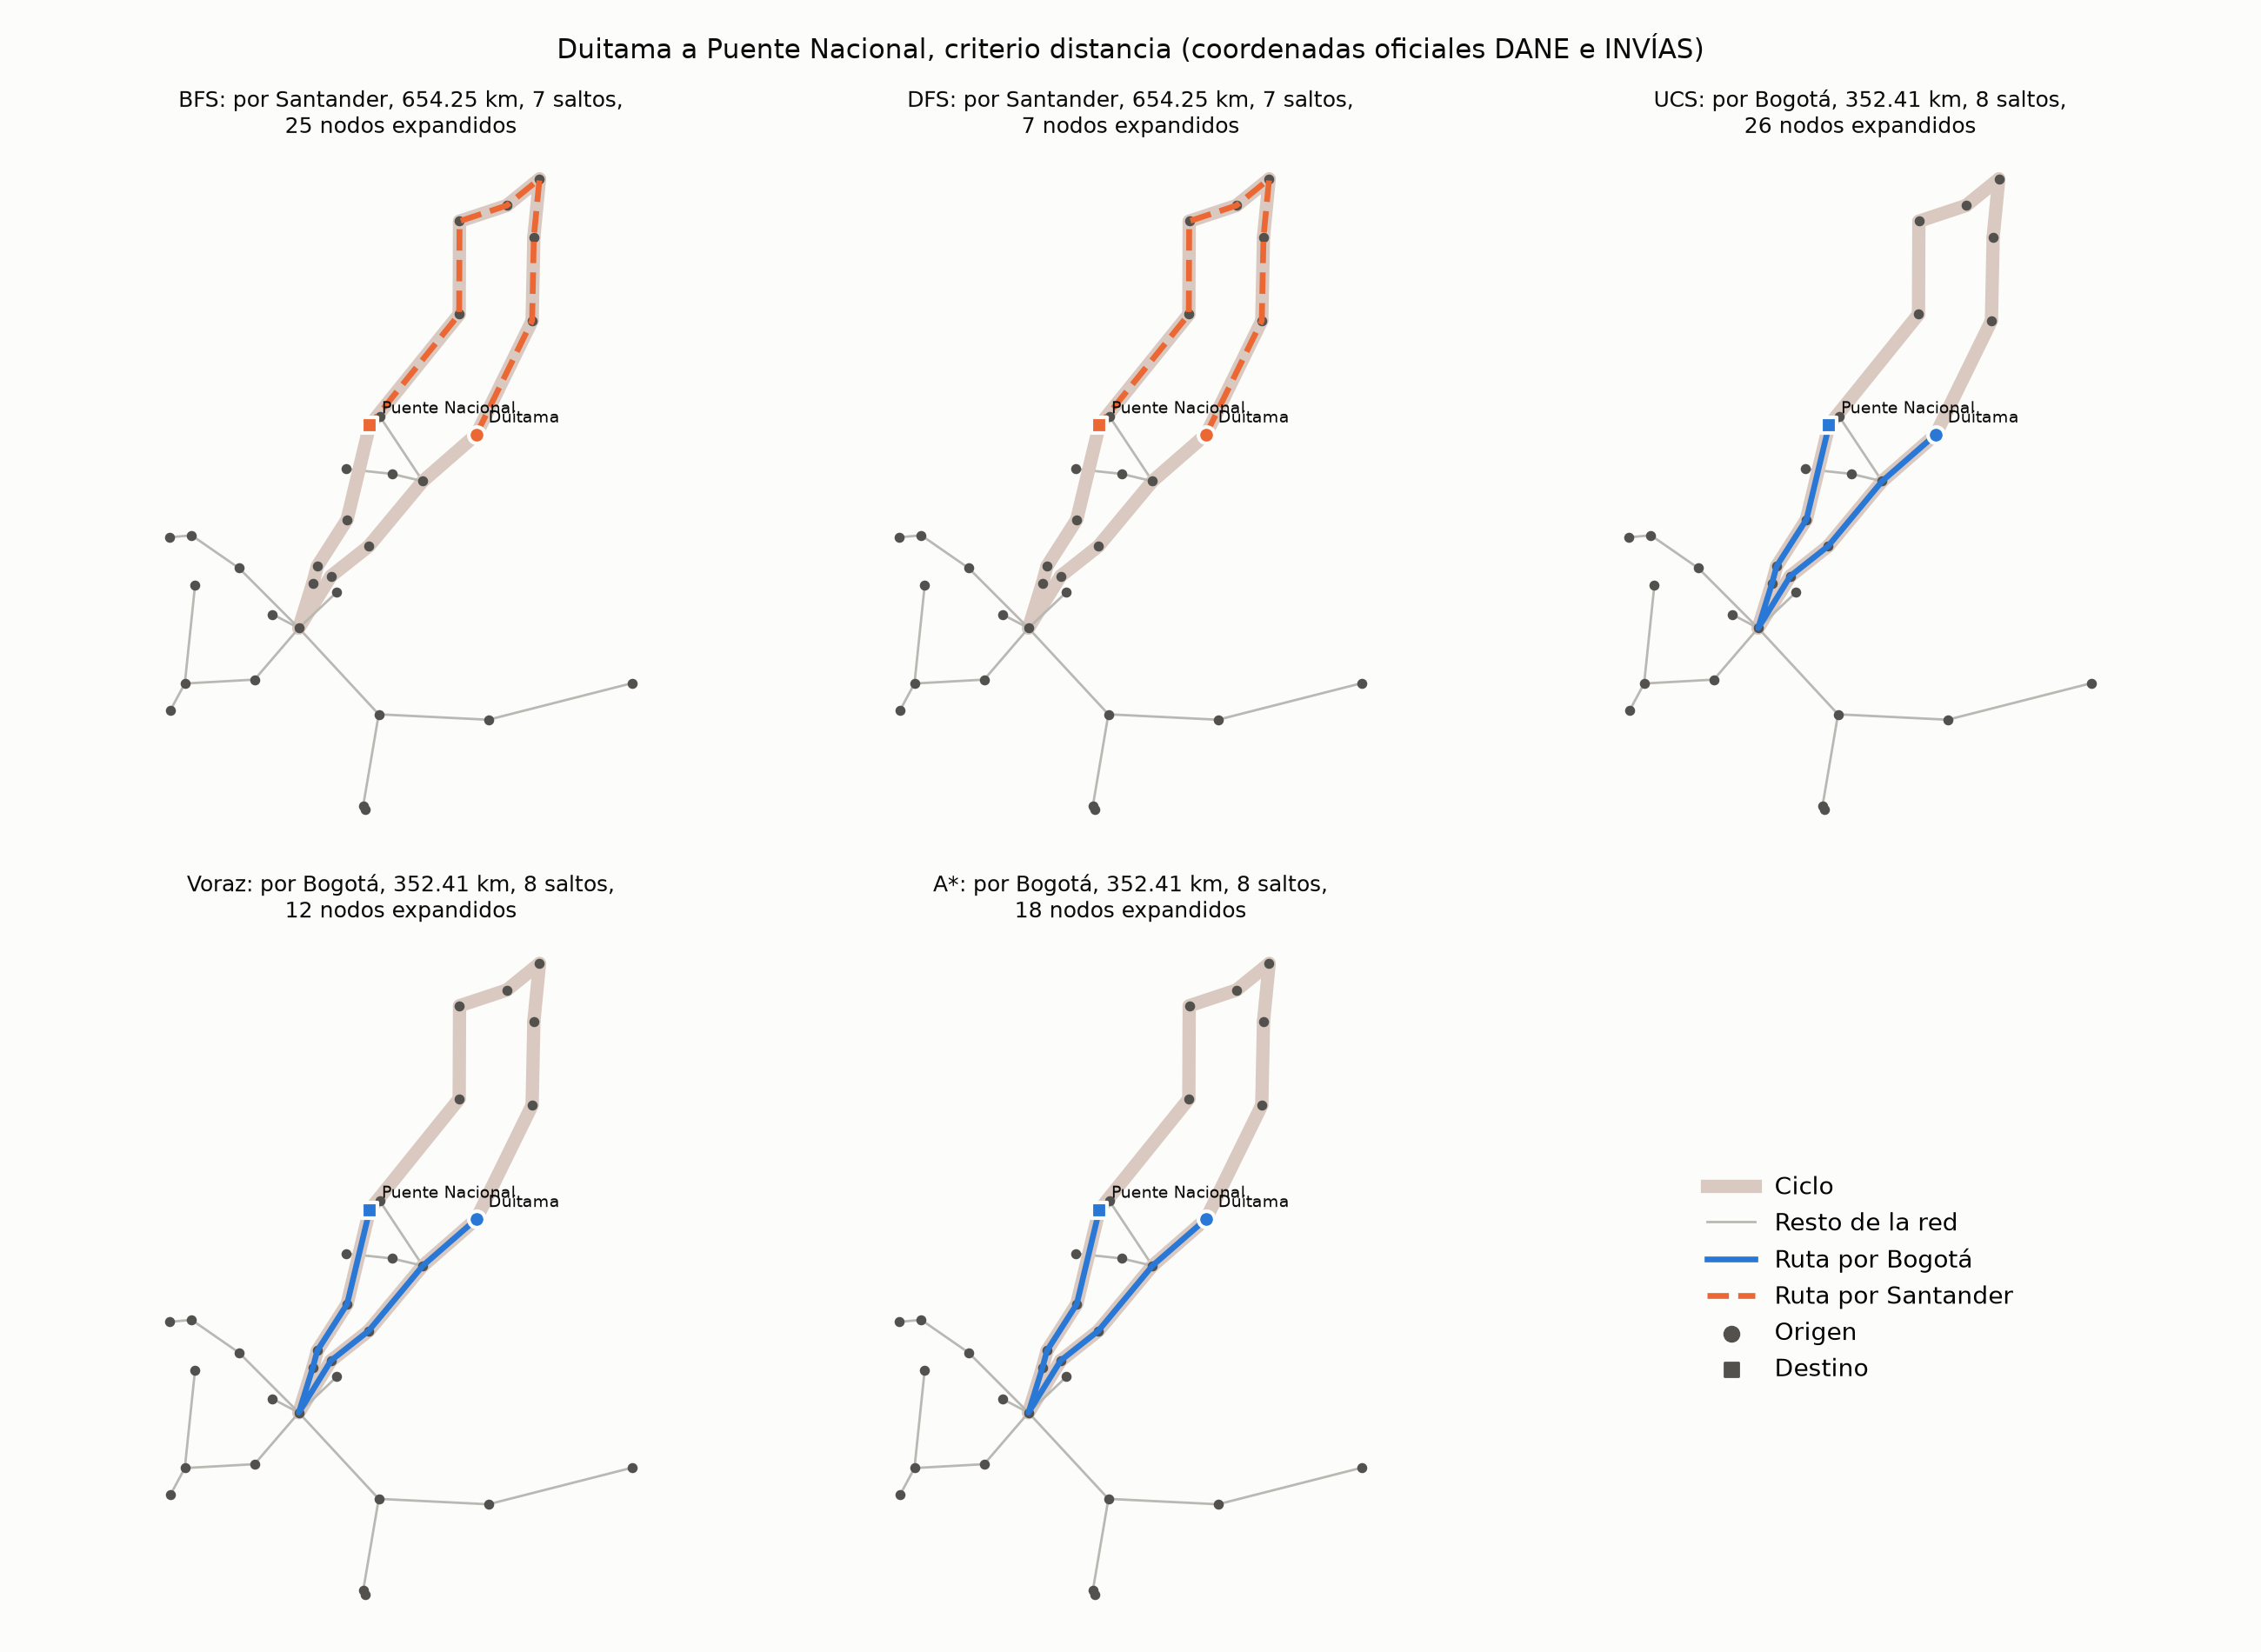
\includegraphics[width=\textwidth]{rutas_central_distancia.png}
    \caption{Rutas de los cinco algoritmos, Duitama a Puente Nacional, criterio
    distancia. Fuente: elaboración propia con datos de INVÍAS y DANE}
    \label{fig:rutas}
\end{figure}

\begin{figure}[H]
    \centering
    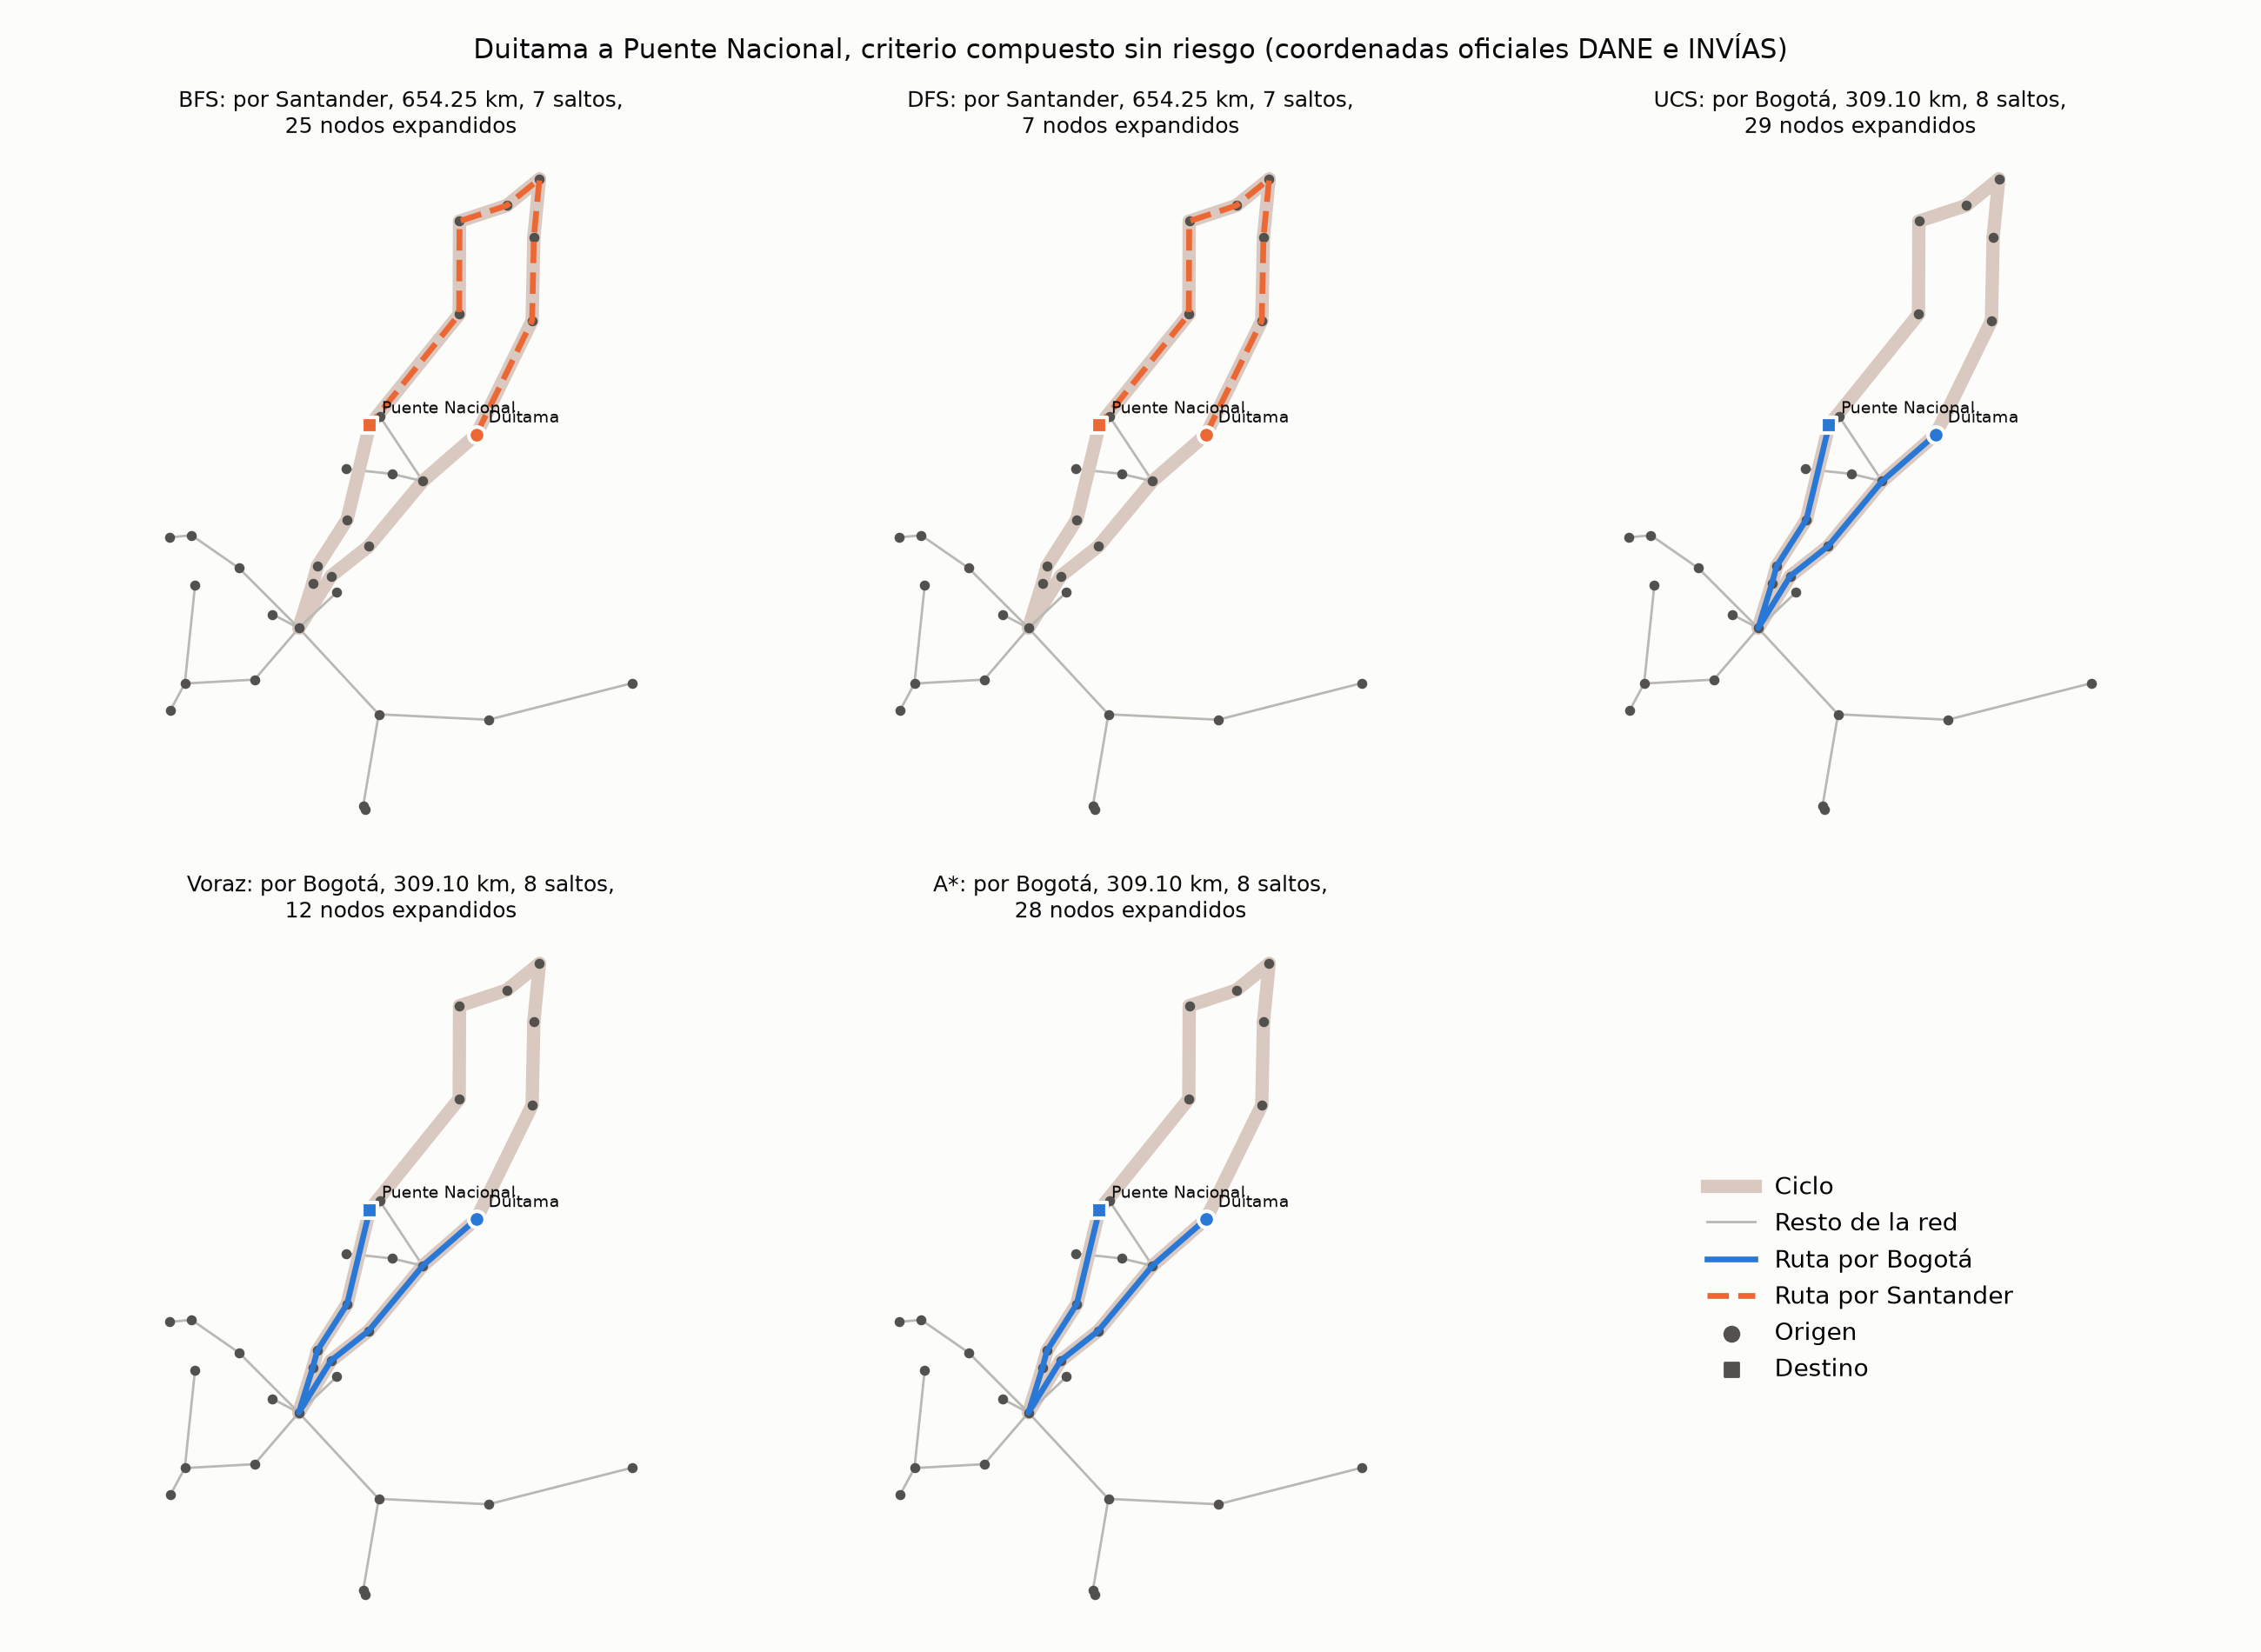
\includegraphics[width=\textwidth]{rutas_central_compuesto_sin_riesgo.png}
    \caption{Rutas de los cinco algoritmos, Duitama a Puente Nacional, criterio
    compuesto sin riesgo. Fuente: elaboración propia con datos de INVÍAS y
    DANE}
    \label{fig:rutas-sr}
\end{figure}

\section{Barrido de pesos}

Para Duitama a Puente Nacional se varió $(w_1, w_2, w_3)$ en una malla de paso
0.1 con suma 1 (66 puntos) y se registró qué ruta gana con el costo compuesto
(riesgo faltante igual a 0). Como solo hay dos rutas simples, el costo de cada
una es lineal en los pesos, $w_1 D + w_2 P + w_3 R$, con $D$, $P$ y $R$ las
sumas de los términos normalizados de la ruta; gana la ruta por Bogotá si
$w_1 \Delta D + w_2 \Delta P + w_3 \Delta R < 0$, con $\Delta$ igual a la ruta
por Bogotá menos la ruta por Santander. En la malla, el ganador de cada punto
coincide con el signo de esta frontera.

\begin{table}[H]
\centering
\caption{Resultado del barrido de pesos}
\label{tab:barrido}
\small
\renewcommand{\arraystretch}{1.2}
\begin{tabular}{|l|r|r|}
\hline
\rowcolor{gray!20} \textbf{Medida} & \textbf{Base} & \textbf{Con cota inferior} \\
\hline
\textbf{Puntos de la malla con ruta por Bogotá (compuesto)} & 19 de 66 & 17 de 66 \\
\hline
\textbf{Puntos con ruta por Bogotá (sin riesgo)} & 37 de 65 & 36 de 65 \\
\hline
\textbf{$w_1$ de cambio sobre $w_3=0$} & 0.4095 & 0.4389 \\
\hline
\textbf{$\Delta D$ (corta menos desvío)} & -2.4477 & -2.1692 \\
\hline
\textbf{$\Delta P$ (corta menos desvío)} & 1.6971 & 1.6971 \\
\hline
\textbf{$\Delta R$ (corta menos desvío)} & 2.8788 & 2.8788 \\
\hline
\end{tabular}

\end{table}

En la red corregida, la ruta por Bogotá gana en 19 de los 66 puntos y la
frontera corta la recta $w_3 = 0$ en $w_1 = 0.4095$; sin el término de riesgo
gana en 37 de los 65 puntos donde esa variante está definida (en
$w_1 = w_2 = 0$ no lo está). La variante \emph{sensibilidad con cota inferior}
reemplaza la distancia de Chocontá a Tunja por 56.96 km: la frontera se
desplaza a $w_1 = 0.4389$, la ruta por Bogotá gana en 17 puntos, y el ganador
cambia en dos puntos de la malla, $(0.5, 0.2, 0.3)$ y $(0.5, 0.3, 0.2)$, que
pasan a Santander. Sin riesgo cambia en un punto, $(0.3, 0.4, 0.3)$.

\begin{figure}[H]
    \centering
    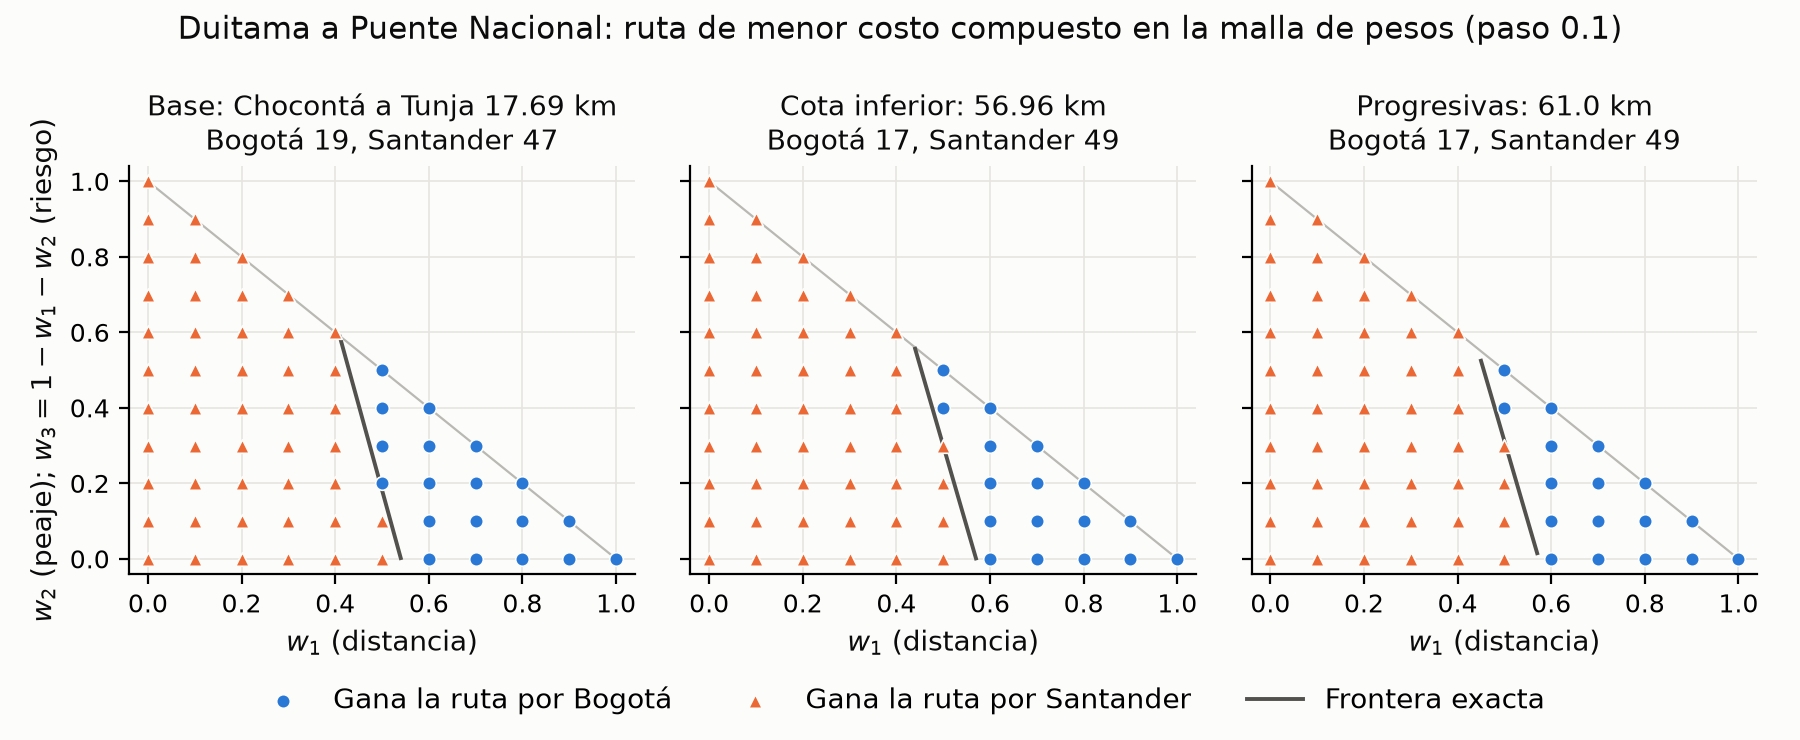
\includegraphics[width=\textwidth]{barrido_pesos.png}
    \caption{Ruta ganadora en la malla de pesos, red corregida y sensibilidad
    con cota inferior. Fuente: elaboración propia}
    \label{fig:barrido}
\end{figure}

\section{Sensibilidad de A* ante el defecto de Chocontá a Tunja}

Variante única, rotulada como sensibilidad: A* con $\alpha_{\mathrm{ref}} =
0.458156$, el mínimo de la razón entre las aristas restantes (sin Chocontá a
Tunja; la determina Madrid a Bogotá). Esta $h$ \emph{no es admisible} en la red
tal como está, porque Chocontá a Tunja tiene razón 0.3106 y $\alpha_{\mathrm{ref}}$
la excede.

\begin{table}[H]
\centering
\caption{Nodos expandidos con $\alpha$ y con $\alpha_{\mathrm{ref}}$,
criterio distancia}
\label{tab:sens-alfa}
\footnotesize\setlength{\tabcolsep}{3pt}
\renewcommand{\arraystretch}{1.2}
\begin{tabular}{|l|r|r|r|c|}
\hline
\rowcolor{gray!20} \textbf{Escenario} & \textbf{UCS} & \textbf{A* $\alpha=0.458156$} & \textbf{A* $\alpha_{\mathrm{reg}}=0.310570$} & \textbf{Óptima} \\
\hline
\textbf{Duitama -- Puente Nacional} & 26 & 18 & 20 & sí \\
\hline
\textbf{Suma de 992 pares} & 15872 & 12361 & 13437 & 992 de 992 \\
\hline
\end{tabular}

\end{table}

A* con $\alpha_{\mathrm{ref}}$ devuelve la ruta óptima en los diez escenarios y
expande menos nodos que con $\alpha = 0.310570$ y que UCS (en el caso central
17, 20 y 25). Sobre los 992 pares de nodos, devuelve la ruta óptima en 991 y
falla en uno: de Bucaramanga a Tunja devuelve 482.01 km frente a un óptimo de
481.34 km (0.14\,\% más). Sumados los 992 pares, UCS expande 15\,872 nodos,
A* con $\alpha$ 13\,377 y A* con $\alpha_{\mathrm{ref}}$ 12\,223.

\section{Discusión}

\begin{itemize}
\item Las rutas de los algoritmos solo difieren en los pares que cruzan el
ciclo: BFS y DFS pueden devolver el desvío, y UCS, A* con $h$ admisible y, en
estos escenarios, la búsqueda voraz devuelven la ruta de menor costo. Con un
solo ciclo, la comparación en los demás pares se limita a nodos expandidos,
tiempo y memoria.
\item A* con heurística admisible expande menos nodos que UCS (120 contra 144
en la suma de los diez escenarios con distancia), pero la ventaja es modesta
porque $\alpha = 0.310570$ hace a $h$ poco informativa.
\item El resultado de los criterios que incluyen el riesgo depende de la
cobertura de los datos: 21 de las 32 aristas no tienen dato de riesgo y valen
0, por lo que \texttt{riesgo} y \texttt{compuesto} prefieren el desvío porque
sus tramos no se midieron, no porque sean más seguros.
\item La corrección de distancias cambia la decisión del criterio compuesto
sin riesgo en el caso central: con las distancias sin corregir elegía el
desvío; con las corregidas elige la ruta por Bogotá (Anexo A).
\end{itemize}

\section{Limitaciones}

\begin{itemize}
\item \textbf{Chocontá a Tunja truncada.} El sector cubre 17.69 km frente a
56.96 km de línea recta; fija $\alpha$ y subestima la ruta por Bogotá (cota
inferior 348.37 km). Las progresivas de la fuente dejan 49.1 km sin registro
entre Chocontá y Tunja; por progresivas la arista mediría 61.0 km, cifra que
solo evidencia que la cota es ajustada y no se aplicó.
\item \textbf{Entrada urbana a Bogotá.} Las geometrías de INVÍAS que salen de
Bogotá empiezan en el límite urbano; las distancias desde Bogotá excluyen ese
tramo.
\item \textbf{Registros con patrón no estándar} (Bogotá a Cajicá, Chocontá a
Tunja, El Espinal a Girardot y el registro del Río Ocoa) conservan la longitud
registrada.
\item \textbf{Riesgo incompleto y por corredor.} Solo 11 de 32 aristas tienen
dato y el dato no distingue subtramos.
\item \textbf{Tarifas de peaje.} Se actualizan cada año; corresponden a la
descarga del 6 de octubre de 2026.
\item \textbf{Mediciones.} El tiempo tiene dispersión alta y la memoria es de
una sola corrida por celda; los valores son indicativos.
\item \textbf{Alcance.} Un solo ciclo, 10 escenarios y 32 nodos.
\end{itemize}

\newpage
\section*{Anexo A: sensibilidad con distancias sin corregir}
\addcontentsline{toc}{section}{Anexo A: sensibilidad con distancias sin
corregir}

La Tabla~\ref{tab:anexo-sens} compara la red corregida (base) con una
variante construida con la longitud registrada (\texttt{shape\_\_length}). Se
genera con la función \texttt{construir\_grafo}, dando el valor
\texttt{cruda} al parámetro \texttt{distancia}, a partir del mismo
\texttt{aristas\_red.json}. La tabla muestra la ruta óptima de Duitama a
Puente Nacional por criterio y el resultado del barrido de pesos.

\begin{table}[H]
\centering
\caption{Sensibilidad: red corregida y distancias sin corregir}
\label{tab:anexo-sens}
\small\setlength{\tabcolsep}{4pt}
\begin{tabular}{lrrrr}
\toprule
\textbf{Criterio} & \textbf{Base: vía} & \textbf{Base: km} & \textbf{Crudas: vía} & \textbf{Crudas: km} \\
\midrule
distancia & Bogotá & 309.10 & Bogotá & 414.84 \\
peaje & Santander & 654.25 & Santander & 668.14 \\
riesgo (limitado) & Santander & 654.25 & Santander & 668.14 \\
compuesto (limitado) & Santander & 654.25 & Santander & 668.14 \\
compuesto sin riesgo & Bogotá & 309.10 & Santander & 668.14 \\
\midrule
Barrido: ruta por Bogotá (compuesto) & \multicolumn{2}{r}{19 de 66} & \multicolumn{2}{r}{12 de 66} \\
Barrido: ruta por Bogotá (sin riesgo) & \multicolumn{2}{r}{37 de 65} & \multicolumn{2}{r}{30 de 65} \\
$w_1$ de cambio sobre $w_3=0$ & \multicolumn{2}{r}{0.4095} & \multicolumn{2}{r}{0.5291} \\
\bottomrule
\end{tabular}

\end{table}

\section*{Anexo B: criterios con heurística limitada}
\addcontentsline{toc}{section}{Anexo B: criterios con heurística limitada}

En \texttt{compuesto} (riesgo faltante igual a 0) la heurística usa solo el
término de distancia; en \texttt{riesgo} es $h = 0$ y A* se reduce a UCS
(los nodos expandidos coinciden). Ambos resultados son limitados.

\begin{table}[H]
\centering
\caption{Nodos expandidos, criterio compuesto (limitado)}
\small\setlength{\tabcolsep}{4pt}
\begin{tabular}{lrrrrr}
\toprule
\textbf{Escenario} & \textbf{BFS} & \textbf{DFS} & \textbf{UCS} & \textbf{Voraz} & \textbf{A*} \\
\midrule
Duitama -- Puente Nacional$^{*}$ & 25 & 7 & 18 & 12 & 17 \\
Tunja -- Ubaté$^{*}$ & 23 & 7 & 17 & 9 & 17 \\
Bucaramanga -- Bogotá$^{*}$ & 12 & 10 & 13 & 6 & 12 \\
Barbosa -- Zipaquirá$^{*}$ & 17 & 6 & 13 & 6 & 13 \\
Bogotá -- Villavicencio & 6 & 24 & 9 & 1 & 6 \\
Girardot -- Cambao & 1 & 1 & 2 & 1 & 2 \\
Chiquinquirá -- Tunja & 2 & 2 & 2 & 2 & 2 \\
Bogotá -- Granada & 19 & 28 & 18 & 3 & 15 \\
Madrid -- Puerto Gaitán & 18 & 26 & 17 & 4 & 14 \\
Mariquita -- Granada & 20 & 31 & 19 & 6 & 17 \\
\bottomrule
\end{tabular}

\end{table}

\begin{table}[H]
\centering
\caption{Optimalidad, criterio compuesto (limitado)}
\small\setlength{\tabcolsep}{3pt}
\begin{tabular}{lrrrrr}
\toprule
\textbf{Escenario} & \textbf{BFS} & \textbf{DFS} & \textbf{UCS} & \textbf{Voraz} & \textbf{A*} \\
\midrule
Duitama -- Puente Nacional$^{*}$ & sí & sí & sí & no ($+30.2\,\%$) & sí \\
Tunja -- Ubaté$^{*}$ & sí & sí & sí & sí & sí \\
Bucaramanga -- Bogotá$^{*}$ & sí & no ($+46.5\,\%$) & sí & sí & sí \\
Barbosa -- Zipaquirá$^{*}$ & sí & sí & sí & sí & sí \\
Bogotá -- Villavicencio & sí & sí & sí & sí & sí \\
Girardot -- Cambao & sí & sí & sí & sí & sí \\
Chiquinquirá -- Tunja & sí & sí & sí & sí & sí \\
Bogotá -- Granada & sí & sí & sí & sí & sí \\
Madrid -- Puerto Gaitán & sí & sí & sí & sí & sí \\
Mariquita -- Granada & sí & sí & sí & sí & sí \\
\bottomrule
\end{tabular}

\end{table}

\begin{table}[H]
\centering
\caption{Nodos expandidos, criterio riesgo (limitado, $h=0$)}
\small\setlength{\tabcolsep}{4pt}
\begin{tabular}{lrrrrr}
\toprule
\textbf{Escenario} & \textbf{BFS} & \textbf{DFS} & \textbf{UCS} & \textbf{Voraz} & \textbf{A*} \\
\midrule
Duitama -- Puente Nacional$^{*}$ & 25 & 7 & 7 & 25 & 7 \\
Tunja -- Ubaté$^{*}$ & 23 & 7 & 12 & 23 & 12 \\
Bucaramanga -- Bogotá$^{*}$ & 12 & 10 & 11 & 12 & 11 \\
Barbosa -- Zipaquirá$^{*}$ & 17 & 6 & 13 & 17 & 13 \\
Bogotá -- Villavicencio & 6 & 24 & 19 & 6 & 19 \\
Girardot -- Cambao & 1 & 1 & 1 & 1 & 1 \\
Chiquinquirá -- Tunja & 2 & 2 & 2 & 2 & 2 \\
Bogotá -- Granada & 19 & 28 & 31 & 19 & 31 \\
Madrid -- Puerto Gaitán & 18 & 26 & 21 & 18 & 21 \\
Mariquita -- Granada & 20 & 31 & 31 & 20 & 31 \\
\bottomrule
\end{tabular}

\end{table}

\begin{table}[H]
\centering
\caption{Optimalidad, criterio riesgo (limitado, $h=0$)}
\footnotesize\setlength{\tabcolsep}{2pt}
\renewcommand{\arraystretch}{1.2}
\begin{tabular}{|l|r|r|r|r|r|}
\hline
\rowcolor{gray!20} \textbf{Escenario} & \textbf{BFS} & \textbf{DFS} & \textbf{UCS} & \textbf{Voraz} & \textbf{A*} \\
\hline
\textbf{Duitama -- Puente Nacional$^{*}$} & sí & sí & sí & sí & sí \\
\hline
\textbf{Tunja -- Ubaté$^{*}$} & no (+259.6\,\%) & no (+259.6\,\%) & sí & no (+259.6\,\%) & sí \\
\hline
\textbf{Bucaramanga -- Bogotá$^{*}$} & sí & no (óptimo $0$, costo 9.854) & sí & sí & sí \\
\hline
\textbf{Barbosa -- Zipaquirá$^{*}$} & no (+259.6\,\%) & no (+259.6\,\%) & sí & no (+259.6\,\%) & sí \\
\hline
\textbf{Bogotá -- Villavicencio} & sí & sí & sí & sí & sí \\
\hline
\textbf{Girardot -- Cambao} & sí & sí & sí & sí & sí \\
\hline
\textbf{Chiquinquirá -- Tunja} & sí & sí & sí & sí & sí \\
\hline
\textbf{Bogotá -- Granada} & sí & sí & sí & sí & sí \\
\hline
\textbf{Madrid -- Puerto Gaitán} & sí & sí & sí & sí & sí \\
\hline
\textbf{Mariquita -- Granada} & sí & sí & sí & sí & sí \\
\hline
\end{tabular}

\end{table}

\section*{Referencias}
\addcontentsline{toc}{section}{Referencias}

\begin{thebibliography}{9}

\bibitem{formulacion}
Andradé Gómez, J. D., Jiménez López, M., y Díaz García, C. A. (2026).
\textit{Formulación del problema y agente de rutas para una red de carga
interurbana} (Proyecto Integrador, Corte 1) [Documento del equipo].
Universidad Sergio Arboleda.

\bibitem{redvial}
INVÍAS. (2026). \textit{Red Vial}. Datos Abiertos Colombia.
\url{https://www.datos.gov.co/Transporte/Red-Vial/ie7y-asdn}

\bibitem{peajes}
INVÍAS. (2026). \textit{Peajes}. Datos Abiertos Colombia.
\url{https://www.datos.gov.co/Transporte/Peajes/68qj-5xux}

\bibitem{siniestralidad}
Agencia Nacional de Seguridad Vial. (2026). \textit{Sectores críticos de
siniestralidad vial}. Datos Abiertos Colombia.
\url{https://www.datos.gov.co/Transporte/SECTORES-CRITICOS-DE-SINIESTRALIDAD-VIAL/rs3u-8r4q}

\bibitem{divipola}
Departamento Administrativo Nacional de Estadística. (2025). \textit{DIVIPOLA:
códigos de municipios y de cabeceras y centros poblados}. Datos Abiertos
Colombia. \url{https://www.datos.gov.co/resource/gdxc-w37w}

\end{thebibliography}

\end{document}
